\chapter{Introduction}
In recent times Convolutional Neural Networks (CNN) have peformed excellent in various fields and thus gained immense popularity. They are advanced feed forward neural networks that are being used in many applications such as image classification, speech recognition etc because of its high accuracy. However, as the architecture of CNNs become more complex, the computation of CNNs become intensive. They require strenuous CPU operations and memory bandwidth, thereby restricting CNN implementation. This demands the need for a dedicated
hardware for its acceleration. Although, Graphics Processing Units (GPU) are conventionally used and provide satisfactory performance on some of the state-of-the-art CNN models, it is not flexible enough to accommodate multiple CNN models. One may need to re-design the entire GPU architecture for a particular CNN. This is where Field Programmable
Gate Arrays (FPGA) prove to be much more beneficial in terms of flexibility
and parallel processing. Apart from the above mentioned advantages, FPGAs can also handle multiple CNNs without changing the structure of the underlying architecture. 

Some state-of-the-art CNN models such as AlexNet,
VGG16 and ResNet have shown considerable performance gain using FPGAs.
Furthermore, the presence of various Software Development Toolkit (SDK)
in the market such as Intel OpenVINO, Xilinx ML Suite and TVM has helped
the developers to efficiently map their CNN models to the underlying architecture. Due to all of these factors, CNN has become a popular choice for image
classification applications.


\section{Why FPGA}
There are multiple hardware available in the market such as CPU, GPU, ASIC, FPGA and each one is used for a specific set of applications. Among all of them FPGAs are becoming widely popular and are being used in CNN based applications. Deep Neural Network (DNN) benefit very much from using FPGA. Since, DNNs are math intensive models, FPGAs can be used to execute the mathematical operations involved in DNNs. FPGAs have dedicated DSPs and ALUs to perform such math intensive floating point arithmetic operations. FPGAs comprise ARM processors and programmable logic for accelerating computing intensive operations. FPGAs are suited for applications which use custom datatypes which is the case in DNN. Also, they provide better latency, parallel processing power and flexibility among all its counterparts. Using FPGA also has another specific advantage. The advantage is that it can accommodate different CNN models without the need of changing the underlying architecture. CNN models have a streaming architecture that suits well with FPGA architecture.
In this project, we have used the Intel Stratix 10 with 520N scaleable FPGA network accelerator card for our CNN inference on image classification. Paderborn Center for Parallel Computing (PC2) has 32 of this FPGA and the primary focus of our task was to scale our CNN architecture using all 32 FPGAs.
Some of the state-of-the-art topologies that have performed exceptionally well in The ImageNet Large Scale Visual Recognition Challenge (ILSVRC) are ResNet and GoogLeNet. Hence, we chose to implement ResNet and GoogleNet and investigated how their performance could be improved through FPGA acceleration while maintaining classification accuracy.
The workload was divided among all the 32 FPGAs and the layers were distributed to each of these FPGAs. Finally, the performance of our system was measured using some performance metrics.

\chapter{Introduction to OpenCL}
OpenCL provides a standard interface for parallel computing and achieves high performance using task and data level parallelism. With OpenCL , you can leverage CPUs, GPUs and other processors as well as DSPs to accelerate parallel computation. OpenCL standard is divided into two parts : a host and a device. Host program is written in C/C++ and runs on CPU. On the device, the language is referred to as kernel code or OpenCL and runs on FPGAs. Kernels provide data parallelism using NDRange launches and provides pipeline parallelism when compiled for an Intel FPGA.
\section{Parallelism using OpenCL features}
\subsection{Loop unrolling}
The basic idea behind loop unrolling is to increase the number of operations per cycle thereby decreasing the number of iterations. At the same time, it also increases the hardware resources. OpenCL provides \#pragma unroll extension
for unrolling loops. To enable loop unrolling specify the syntax \#pragma unroll[unroll factor].
\begin{figure}[!htb]
    \centering
    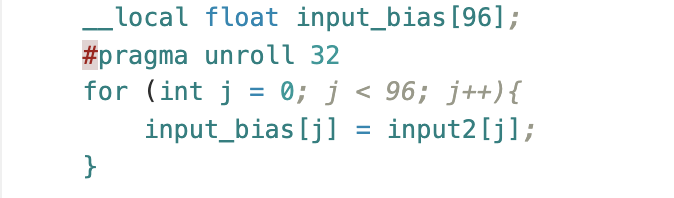
\includegraphics[width=\textwidth,height=\textheight,keepaspectratio]{img/Loop_unrolling.png}
    \caption{Loop unrolling}
    \label{Loop unrolling}
\end{figure}
<\newpage>
\subsection{Pipelining}
Pipelining enables pipeline parallelism. Basically without pipelining, each instruction is processed from start to finish before moving on to the next. But Pipelining allows the various hardware sections to each process a different instruction simultaneously.
\begin{figure}[h!]
    \centering
    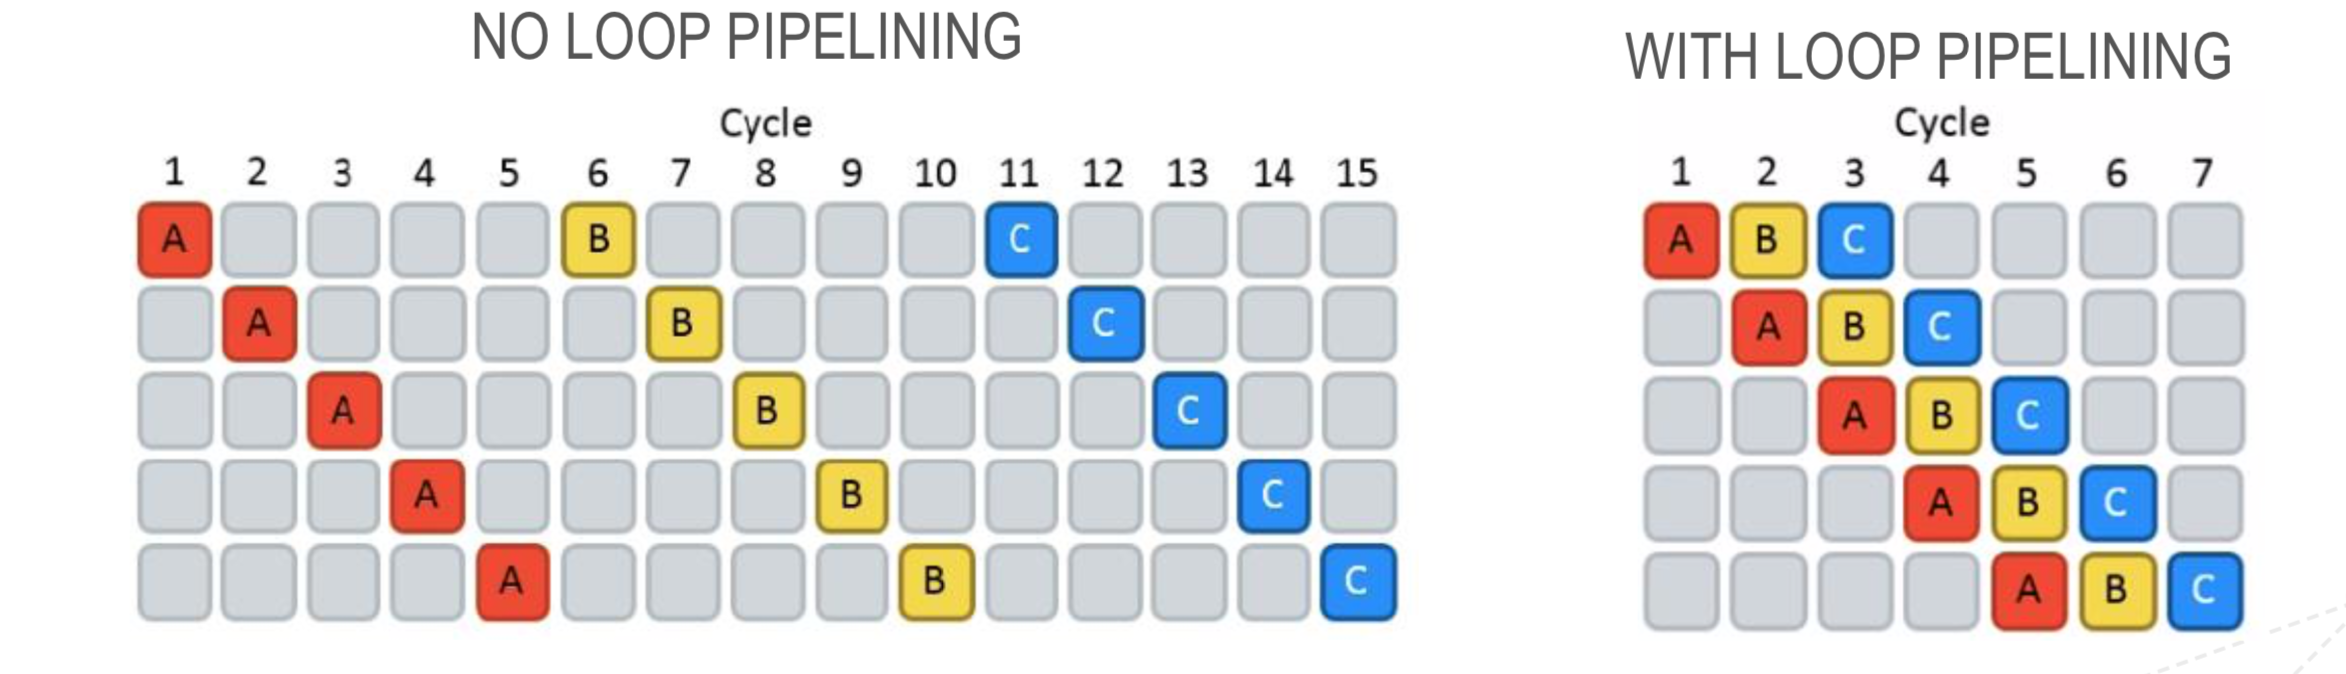
\includegraphics[scale=0.4]{img/Pipelining.png}
    \caption{Pipelining}
\end{figure}